
\documentclass[12pt,letterpaper]{article}
\usepackage[utf8]{inputenc}
\usepackage[spanish]{babel}
\usepackage{graphicx}
\usepackage[hidelinks]{hyperref}
\usepackage{hyperref}
\usepackage[left=2cm,right=2cm,top=2.5cm,bottom=2cm]{geometry}
\usepackage{graphicx} % figuras
\usepackage{float} % para usar [H]
\usepackage{amsmath}
\usepackage{stackrel} 
\usepackage{multicol}
\usepackage{multirow}
\usepackage{fancyhdr}
\usepackage[usenames,dvipsnames,svgnames,table]{xcolor}
\usepackage[document]{ragged2e}
\usepackage{enumerate} % enumerados
\renewcommand{\labelitemi}{$-$}
\renewcommand{\labelitemii}{$\cdot$}

\begin{document}
	\begin{titlepage}
		\begin{center}
			\begin{figure}[htb]
				\begin{center}
					
\includegraphics[width=3.5cm]{./img/upt}
				\end{center}
			\end{figure}
			\vspace*{0.15in}
			\begin{Large}
				\textbf{UNIVERSIDAD PRIVADA DE TACNA}\\
			\end{Large}
			\vspace*{0.15in}
			\begin{Large}
				\textbf{FACULTAD DE INGENIERIA} \\
			\end{Large}
			\vspace*{0.1in}
			\begin{Large}
				\textbf{Escuela Profesional de Ingeniería de Sistemas} \\
			\end{Large}
			\vspace*{0.3in}
			\begin{Large}
				\textbf{INFORME DE LABORATORIO N°03}\\
				\textbf{“MongoDB on AWS”}\\
			\end{Large}
			\vspace*{0.2in}
			\begin{Large}
				\textbf{CURSO:} \\
			\end{Large}
			\vspace*{0.1in}
			\begin{large}
				Base de Datos II\\
			\end{large}
			\vspace*{0.2in}
			\begin{Large}
				\textbf{DOCENTE:} \\
			\end{Large}
			\vspace*{0.1in}
			\begin{large}
				Ing. Patrick Jose Cuadros Quiroga\\
			\end{large}
			\vspace*{0.3in}
			\begin{large}
				\textbf{ALUMNO:} \\
				\begin{flushleft}
					Risther Jaime Tarqui Montalico  		\hfill	(2017057469) \\
				\end{flushleft}
			\end{large}
			\vspace*{1.3in}
			\begin{large}
				Tacna - Perú\\
			\end{large}
			\vspace*{0.1in}
			\begin{large}
				2020\\
			\end{large}
		\end{center}
	\end{titlepage}
	\include{Secciones/articulo}
	\newpage
	
	\justify
	
	\begin{LARGE}
		\begin{center}
			\textbf{MongoDB on AWS} \\
		\end{center}
	\end{LARGE}
	\section{OBJETIVO}
	\begin{itemize}
		\item Configurar un clúster MongoDB totalmente personalizable a pedido,analizar la construcción de una infraestructura escalable y bajo demanda en AWS que proporciona una solución rentable para manejar los requisitos de almacenamiento y computación a gran escala. 
	\end{itemize}
	
	\section{DESARROLLO}

	
	\subsection{Paso 1. Prepare la cuenta}
\item	Puede implementar MongoDB fácilmente en la plataforma flexible de AWS. Esta guía sirve como referencia para los clientes que desean configurar un clúster MongoDB totalmente personalizable a pedido. La construcción de una infraestructura escalable y bajo demanda en AWS proporciona una solución rentable para manejar los requisitos de almacenamiento y computación a gran escala. La arquitectura flexible de AWS le permite elegir la infraestructura de red, computación y almacenamiento más adecuada para su entorno.
	\begin{enumerate}
		
		\item Si aún no tiene una cuenta de AWS, cree una en https://aws.amazon.comsiguiendo las instrucciones en pantalla. Parte del proceso de registro implica recibir una llamada telefónica e ingresar un PIN usando el teclado del teléfono.
		\begin{center}
			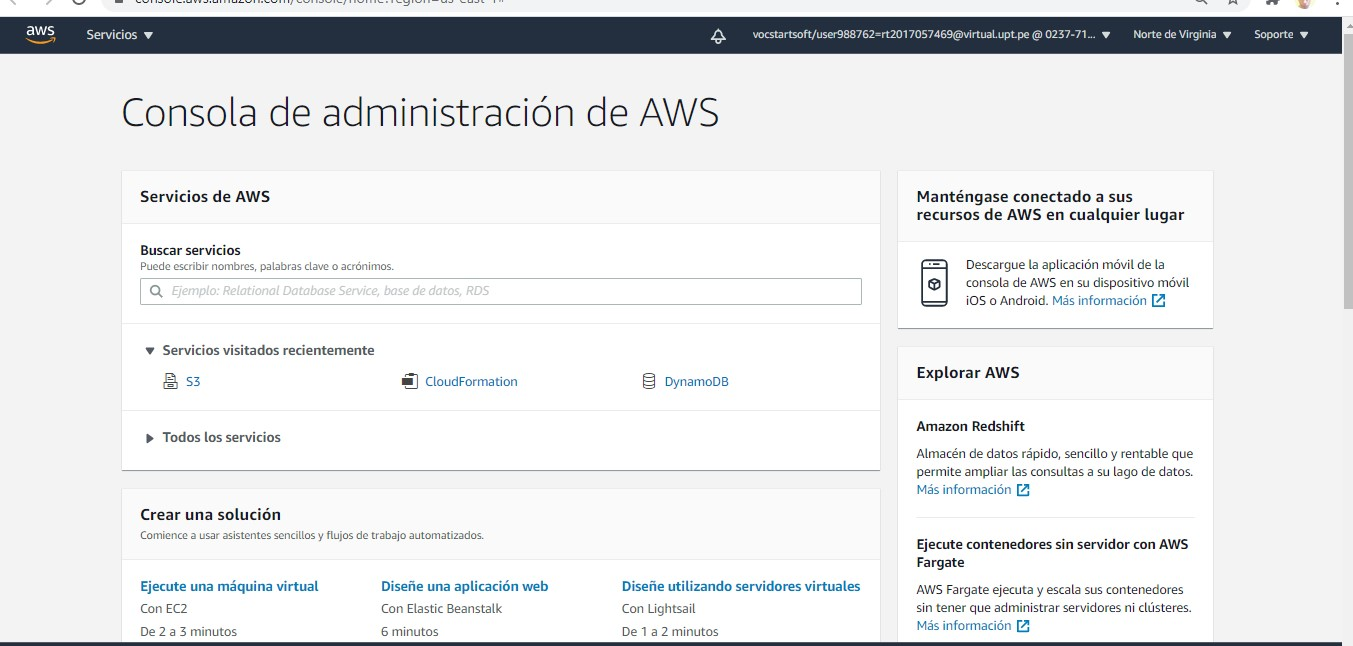
\includegraphics[width=14cm]{./img/1.1.jpg} 
		\end{center}
		\item Utilice el selector de región en la barra de navegación para elegir la región de AWS donde desea implementar el clúster de MongoDB en AWS. Para obtener más información, consulte Regiones, zonas de disponibilidad y zonas locales . Las regiones están dispersas y ubicadas en áreas geográficas separadas. Cada región incluye al menos dos zonas de disponibilidad que están aisladas entre sí pero conectadas a través de enlaces de baja latencia.
		\begin{center}
			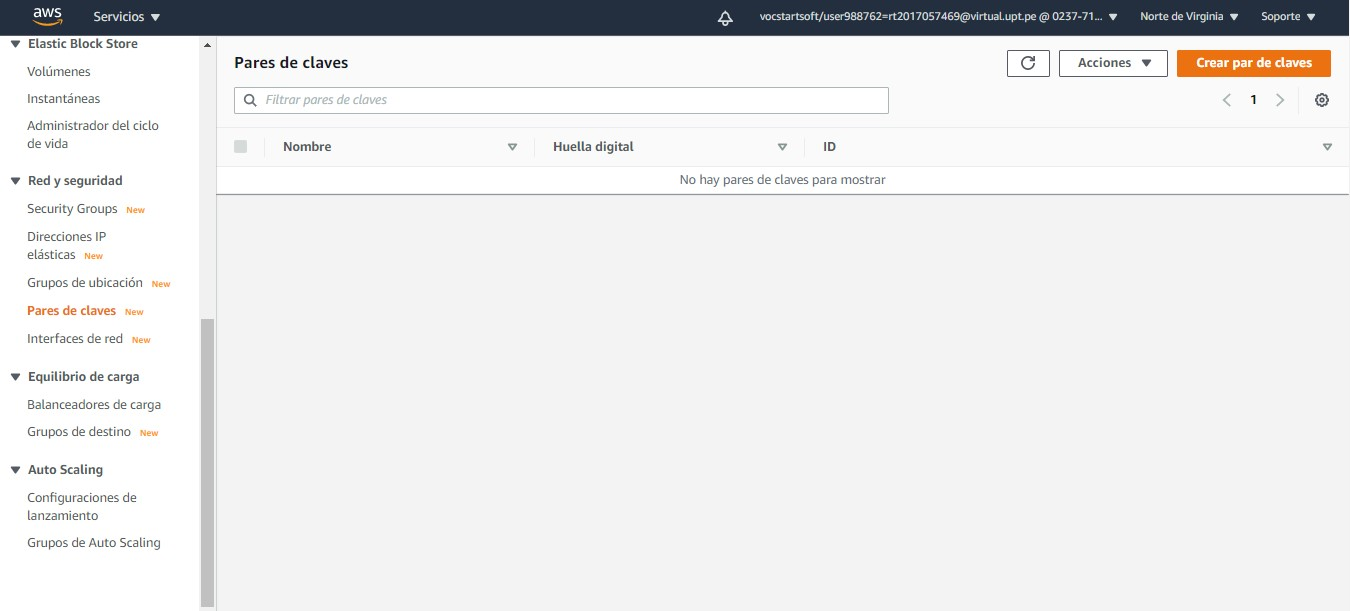
\includegraphics[width=14cm]{./img/1.2.1.jpg} 
		\end{center}
		\begin{center}
		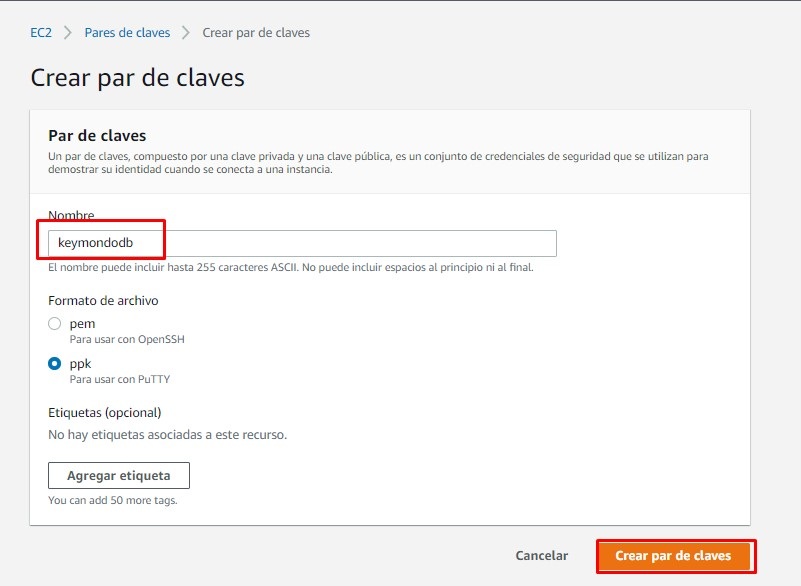
\includegraphics[width=14cm]{./img/1.2.2.jpg} 
	\end{center}

		\item  Cree un par de claves en su región preferida. Para ello, en el panel de navegación de la consola de Amazon EC2, elija Key Pairs , Create Key Pair , escriba un nombre y luego elija Create .
		\begin{center}
			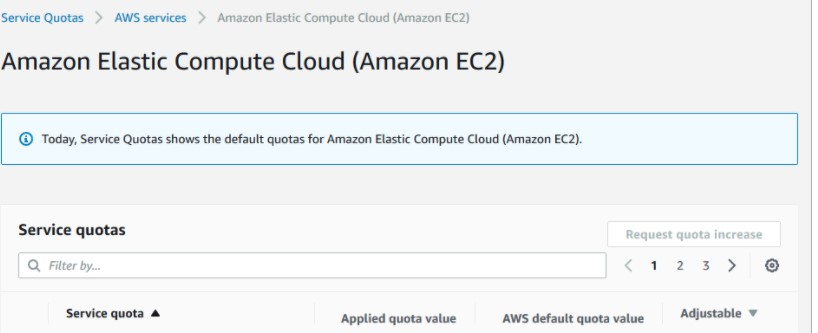
\includegraphics[width=14cm]{./img/1.3.jpg} 
		\end{center}
	         Si es necesario, solicite un aumento de la cuota de serviciopara los tipos de instancias de Amazon EC2 que desea implementar. Para hacer esto, en la consola de Cuotas de servicio, para cada tipo de instancia que desee un aumento de cuota de servicio, elija el tipo de instancia, elija Solicitar aumento de cuota y luego complete los campos en el formulario de aumento de cuota.
	         
	    \item      La cuota predeterminada para el número de instancias depende del tipo de instancia que elija y actualmente varía de 2 a 20 (consulte la página de preguntas frecuentes de Amazon EC2). Si tiene implementaciones existentes que también usan este tipo de instancia, o si planea superar el valor predeterminado con esta implementación de referencia, deberá solicitar un aumento de la cuota. Es posible que la nueva cuota de servicio demore unos días en entrar en vigencia. Para obtener más información, consulte la documentación de AWS .
	    
	    \item Si es necesario, solicite un aumento de la cuota para las direcciones IP elásticas en la VPC. Elija Número de EIP - VPC EIP para la cuota de servicio , elija Solicitar aumento de cuota y complete los campos en el formulario de solicitud de cuota.
	    \item Si es necesario, solicita un aumento de cuotapara los volúmenes de EBS que puede utilizar. Elija el tipo de volumen, elija Solicitar aumento de cuota y complete los campos en el formulario de solicitud de cuota.
	    
	    
\subsection{Paso 2. Inicie el inicio rápido }
		
	\begin{enumerate}
		
		\item Elija una de las siguientes opciones para iniciar la plantilla de AWS CloudFormation en su cuenta de AWS. Para obtener ayuda para elegir una opción, consulte Opciones de implementación anteriormente en esta guía.
	\\	d. Elija Create cluster.
		\begin{center}
			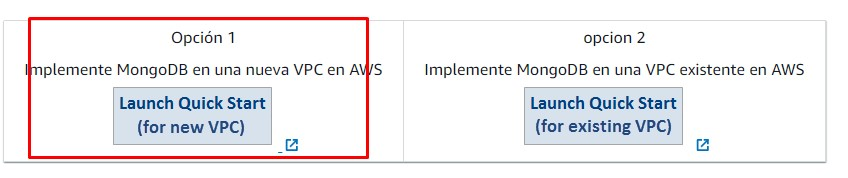
\includegraphics[width=14cm]{./img/2.1.jpg} 
		\end{center}
		\item Compruebe la región que se muestra en la esquina superior derecha de la barra de navegación y cámbiela si es necesario. La plantilla se lanza en la región de EE.UU.Este (Norte de Virginia) de forma predeterminada.
		\begin{center}
			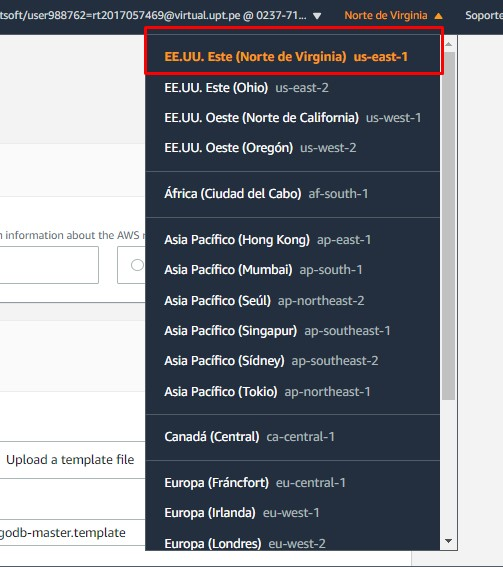
\includegraphics[width=14cm]{./img/2.2.jpg} 
		\end{center}
		\item En la página Seleccionar plantilla , mantenga la configuración predeterminada para la URL de la plantilla y luego elija Siguiente .
		
		\begin{center}
			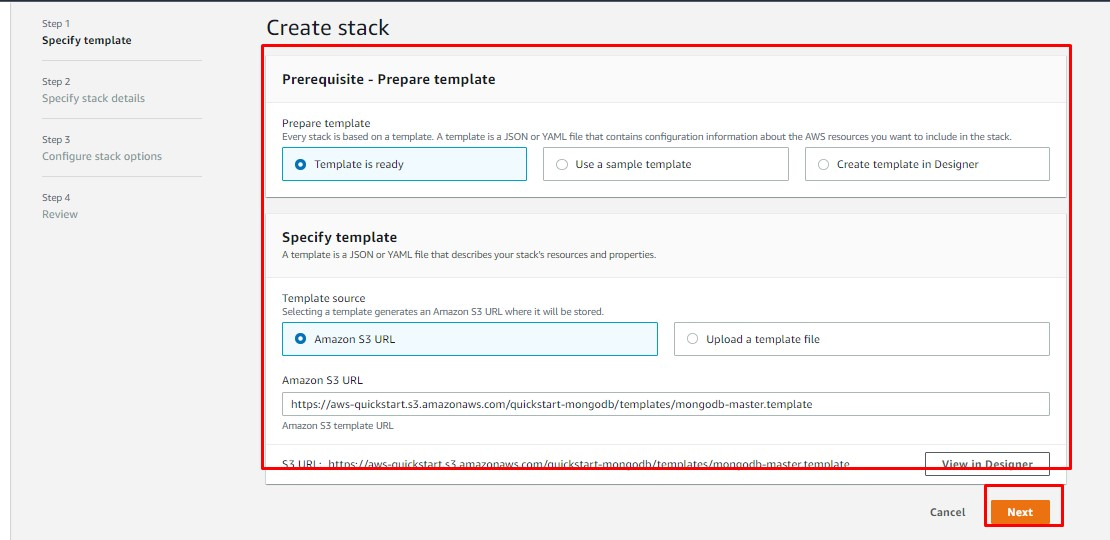
\includegraphics[width=14cm]{./img/2.3.jpg} 
		\end{center}
		\item En la página Especificar detalles , cambie el nombre de la pila si es necesario. Revise los parámetros de la plantilla. Proporcione valores para los parámetros que requieren su entrada. Para todos los demás parámetros, revise la configuración predeterminada y personalícela según sea necesario. Cuando termine de revisar y personalizar los parámetros, elija Siguiente .
		
		En las siguientes tablas, los parámetros se enumeran por categoría y se describen por separado para las dos opciones de implementación:
		
		\begin{center}
			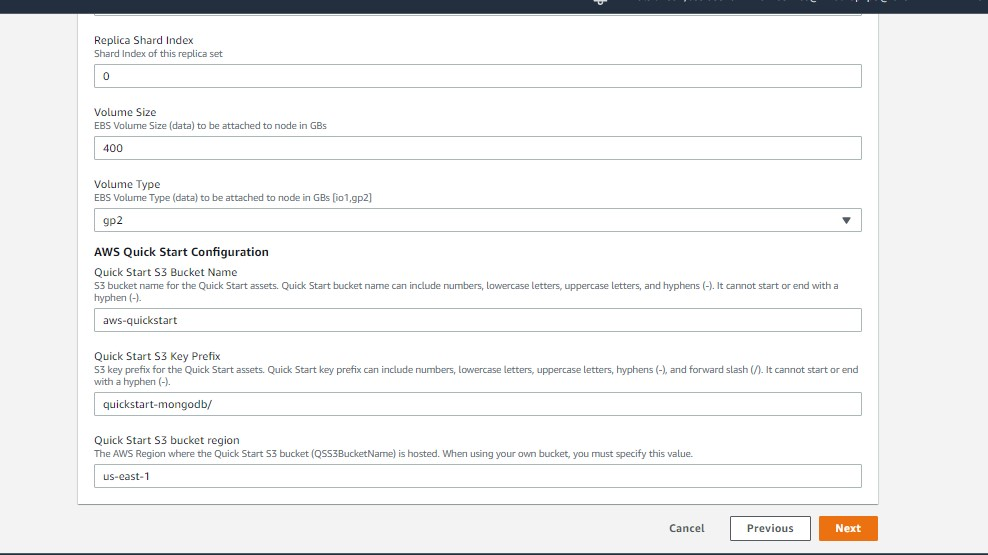
\includegraphics[width=14cm]{./img/2.4.jpg} 
		\end{center}
		\item En la página Opciones , puede especificar etiquetas (pares clave-valor) para los recursos en su pila y establecer opciones avanzadas . Cuando haya terminado, elija Siguiente .
		\begin{center}
			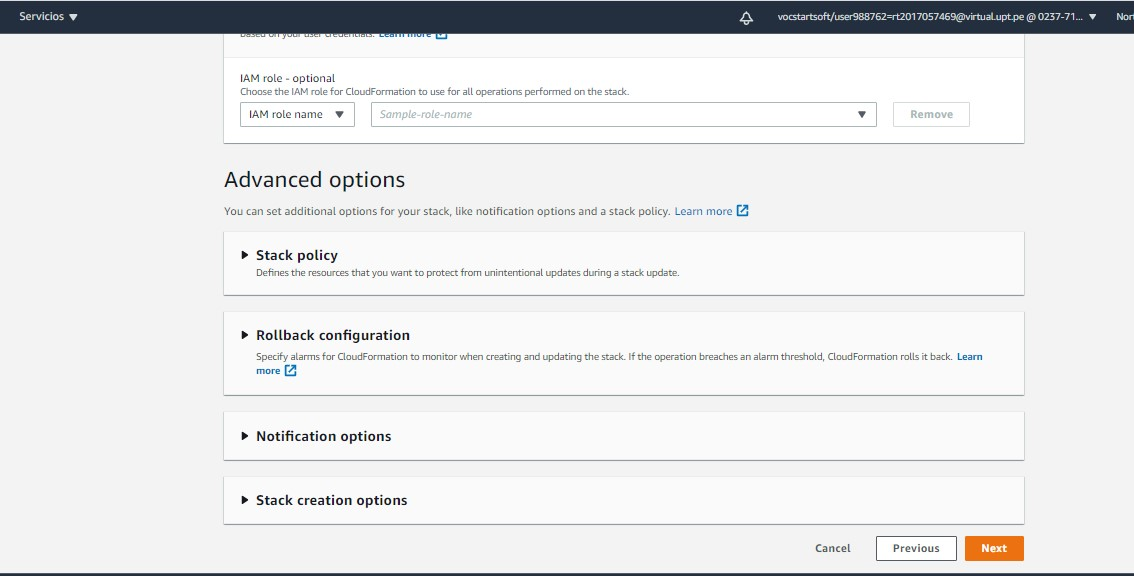
\includegraphics[width=14cm]{./img/2.5.jpg} 
		\end{center}
	\begin{center}
		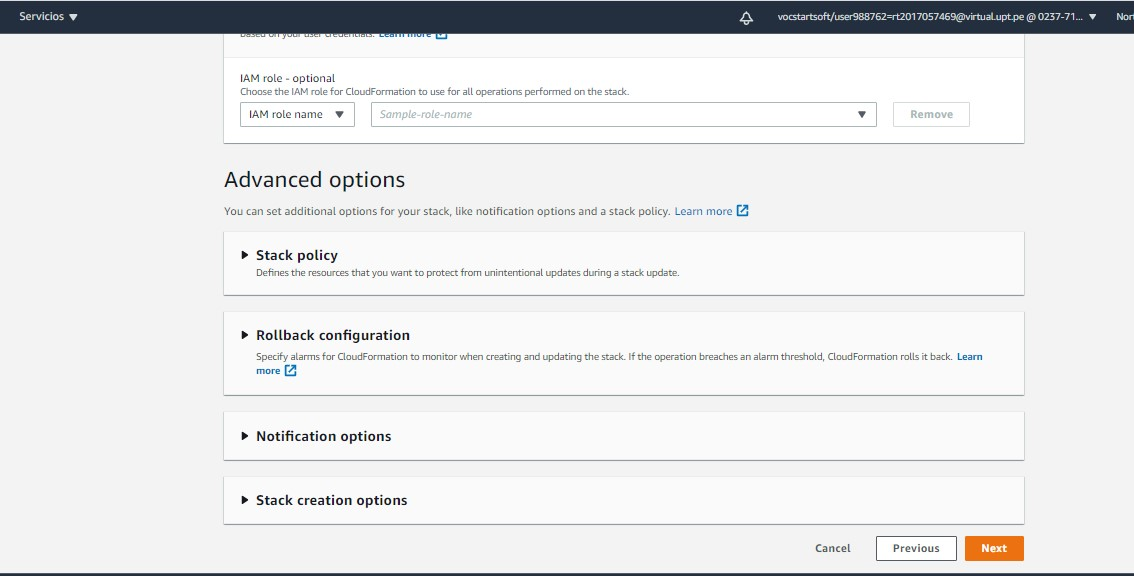
\includegraphics[width=14cm]{./img/2.5.jpg} 
	\end{center}
		\item Elija Crear para implementar la pila.
		\item Supervise el estado de la pila. Cuando el estado es CREATE_COMPLETE , como se muestra en la Figura 6, el clúster de MongoDB está listo.
		\begin{center}
			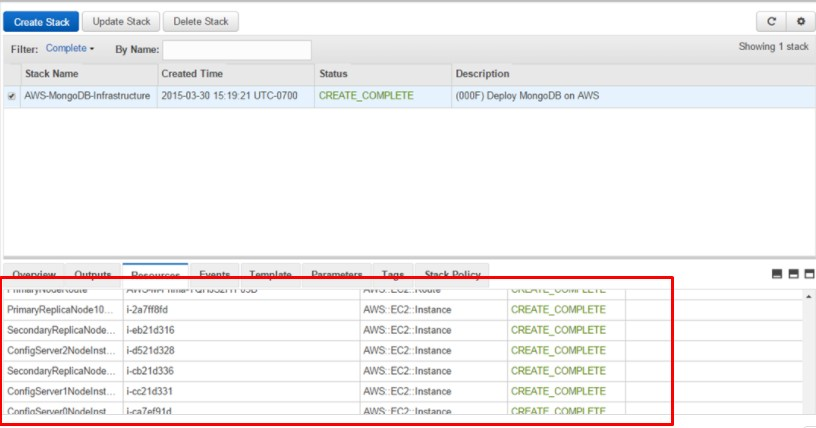
\includegraphics[width=14cm]{./img/2.8.jpg} 
		\end{center}
		
		\end{enumerate}
	\subsection{Paso 3. Conéctese a los nodos de MongoDB }


	\begin{enumerate}
		
		\item Una vez que la plantilla de AWS CloudFormation haya creado correctamente la pila, todos los nodos de MongoDB se ejecutarán con el software instalado en su cuenta de AWS. Para conectarse a cualquiera de los nodos de MongoDB, use SSH para conectarse a la instancia de host bastión. En la consola de Amazon EC2, elija la instancia y luego elija Connect .
	\begin{center}
		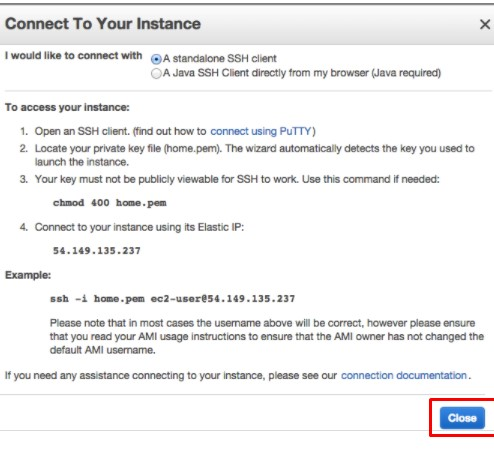
\includegraphics[width=14cm]{./img/3.1.jpg} 
	\end{center}
		\item Una vez que se conecte a la instancia de host bastión mediante SSH, puede conectarse a cualquiera de los nodos de MongoDB de manera similar (elija el nodo y luego elija Conectar para encontrar el comando SSH). 

		\begin{center}
			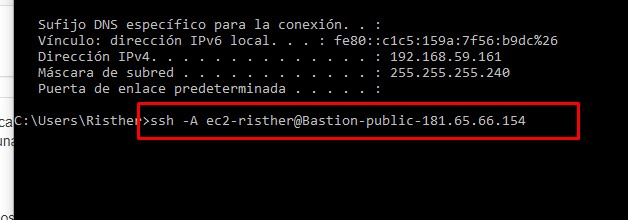
\includegraphics[width=14cm]{./img/3.2.jpg} 
		\end{center}
		\item
		 Tenga en cuenta que todos los nodos de MongoDB se lanzan con un rol de IAM que les otorga privilegios para crear y eliminar tablas de Amazon DynamoDB, acceder a Amazon Simple Storage Service (Amazon S3), crear y eliminar instancias de Amazon EC2, etc. Puede modificar la política mediante la consola de IAM. Para obtener detalles sobre los beneficios de los roles de IAM, consulte Uso de roles de IAM para delegar permisos a aplicaciones que se ejecutan en Amazon EC2 en la documentación de AWS. 
	
	
		\end{enumerate}
		
	\section{CONCLUSIONES}
	\begin{itemize}
			\item Se realiza creacion de key para MongoDB y analizamos la infraestructura escalable demanda de AWS.Finalmente se realizo la implementacion del MongoDB en AWS.
			
		\end{itemize}
		
		
	\end{document}